\chapter[Smooth]{Constructive proof that a smooth, closed, orientable 3--manifold is the boundary of some 4--manifold}
\label{chapter:smooth}

We prove that every smooth, closed, orientable 3--manifold is the boundary of some 4--manifold.
We do so by explicitly constructing such a 4--manifold from a given 3--manifold.
This construction is mirrored in Chapter \ref{chapter:triangulation} where we prove the same for a given closed, orientable 3--manifold triangulation and provide an algorithm.

Let $M$ be a smooth, closed, orientable 3--manifold and take $W=M\times \Ilit$.
Then $W$ is a 4--manifold with boundary
\[
	\pd W = (M\times\{0\}) \cup (M\times\{1\}) = M_0 \cup M_1.
\]
We construct a manifold with only one boundary component from $W$ by attaching 4--dimensional 2--, 3--, and 4--handles to $W$ over the part of its boundary away from $M_0$.
We start by attaching 2--handles to $W$ over $M_1$ to produce a 4--manifold $W'$ with boundary $M_0 \sqcup M_1'$, where $M_1'=\pd W'\setminus M_0$ and is described via surgery on $M_1$.
We then attach 3--handles to $W'$ over $M_1'$ to produce a 4--manifold $W''$ with boundary $M_0\sqcup M_1''$.
As before, $M_1''=\pd W''\setminus M_1$ and $M_1''$ is described via surgery on $M_1'$.
At this point in the construction, $M_1''$ is the disjoint union of a finite number of copies of $S^3$.
We attach 4--handles to $W''$ over $M_1''$ to produce a 4--manifold whose boundary is exactly $M_0$.

Instructions for handle attachment come from defining a projection $f:M_1\to \RR$ that induces a stratification of $M_1\subset\pd W$.

%
% indexed partially by dimension of the pure strata as a submanifold of $M_1$.
% such that each closed stratum $M_1^3$ is a disjoint collection of open submanifolds of $M_1$.
%
We call a closed 3--dimensional stratum of $M_1$ a \emph{block}, and we impose conditions on $f$ to ensure that every block can be classified up to \emph{stratified homeomorphism}.
We say that $X,Y$ are \emph{stratified homeomorphic} if $X,Y$ are stratified spaces and there exists a homeomorphism $f:X\to Y$ such that $f$ and $f\inv$ are each stratified maps.
The blocks of $M_1$ are described below:

\begin{itemize}
	\item \emph{face block}:
		An attachment neighbourhood for a stratified 2--handle.
		Each face block is stratified-homeomorphic to $S^1\times G_n$, the product of the circle with an $n$-gon for some $n$.
	
	\item \emph{edge block}:
		A partial attachment neighbourhood for a stratified 3--handle.
		Each edge block is stratified-homeomorphic to one of $D^2\times\Ilit$, $A\times\Ilit$, or $P\times\Ilit$, where $A$ is the annulus $S^1\times\Ilit$ and $P$ is a pair-of-pants surface.
		Attachment of stratified (4,2)--handles over our face blocks ``fill in'' the annular boundary components of edge blocks, forming full attachment neighbourhoods for stratified 3--handles.
		
	\item \emph{vertex block}:
		A partial attachment neighbourhood for a stratified 4--handle.
		Each vertex block is homeomorphic to a (3,1)-handlebody of genus at most 3.
		When stratified (4,2)-- and (4,3)--handles are attached to $W$, the genus of these handlebodies are reduced until the remaining boundary of $W$ consists of $M_0$ union a collection of stratified 3--spheres.  The 3--spheres are then coned away.
\end{itemize}
 
The remainder of this chapter is spent ensuring that such a stratification can be achieved for any smooth, orientable, closed 3--manifold, detailing how the stratification is induced, proving that the attachment of stratified (4,2)-- and (4,3)--handles has the previously stated effects, and discussing the resulting 4--manifold.

\section{Projections from 3--manifolds to $\RR$}
\label{section:smooth-projection}

Our stratification of $M$ is induced by a decomposition of the plane, itself induced by the singular values of a smooth map $M\to\RR$.
To prove that a stratification suitable for our construction exists for any smooth orientable 3--manifold, we show first that an inducing decomposition of $\RR$ exists.
To prove that such a decomposition of $\RR$ exists, we present the properties of $f:M\to\RR$ required to induce the decomposition, and argue why a map possessing such properties exists for any smooth, orientable 3--manifold.

Let $f:M\to\RR$ be a smooth map, let $df$ be the differential of $f$, and let $S_r(f)$ be the set of points in $M$ such that $df$ has rank $r$.
Then we require that the following be true of $f$:
\begin{enumerate}
	\item $S_0(f)$ is empty.
	
	\item $S_1(f)$ consists of smooth non-intersecting curves.  We call these the \emph{fold curves} of $f$.
	
	\item The set of points where $f|_{S_1(f)}$ has zero differential (these can appear in the image of $S_1(f)$ as cusps in the plane) is empty.
	
	\item Let $\gamma_i, \gamma_j, \gamma_k \in S_1(f)$ be fold curves. Then $f(\gamma_{i,j,k})$ are submanifolds of $\RR$ such that
	\begin{enumerate}
		\item $f(\gamma_i)$ and $f(\gamma_j)$ intersect transversely,
		
		\item $f(\gamma_i)\cap f(\gamma_j)\cap f(\gamma_k)$ is empty (i.e. there are no triple-intersections), and
		
		\item self-intersections of $f(\gamma_i)$ are transverse
	\end{enumerate}
	
	\item If $p\in S_1(f)$ then there exist coordinates $(u, z_1, z_2)$ centred at $p$ and $(x,y)$ centred at $f(p)$ such that $f$ takes the form of either
	\begin{enumerate}
		\item\label{property:paraboloid} $(x,y)=(u,\pm(z_1^2+z_2^2))$, or
		\item\label{property:saddle} $(x,y)=(u,\pm(z_1^2-z_2^2))$
	\end{enumerate}
	in a neighbourhood of $p$.
	If $f$ takes the form of \ref{property:paraboloid} then we further classify $p$ as a \emph{definite fold}, and if $f$ takes the form of \ref{property:saddle} then $p$ is an \emph{indefinite fold}.
	
	\item The set of singular values of $f$ in the plane is connected
	
	\item $f(M)$ is bounded.
\end{enumerate}

The first four conditions ensure that the set of singular values in the plane is well-behaved, the fifth allows classification of singular fibers of $f$ using the work of Saeki \cite{Saeki}, and the sixth guarantees that the set of singular values of $f$ partitions the image of $M$ into discs.
We call these five conditions the \emph{stratification conditions} on $f$.

\section{Stratifying $\RR$}
\label{section:smooth-decompose}

Let $f:M\to\RR$ be a smooth map possessing the stratification conditions of Section \ref{section:smooth-projection} and let $X_f = f(S(f))$, the set of singular values of $f$.
$X_f$ is a connected collection of arcs in the plane that intersect only transversely.

We fit closed neighbourhoods (\emph{sleeves}) around the singular values of $f$ and classify these sleeves by the maximum codimension (with respect to $\RR$) of singular values they contain.
Because $X_f$ consists of codimension 1 and codimension 2 singular values (i.e.\ arcs and arc-crossings respectively), we stratify $\RR$ into face regions that contain no singular values, edge regions that contain only codimension 1 singular values, and vertex regions, each of which contain exactly 1 codimension 2 singular value.
Figures \ref{fig:vertex-sleeve}-\ref{fig:face-sleeve} are used to illustrate the stratification resulting from sleeve-fitting.

\begin{figure}[h!]
	\centering
	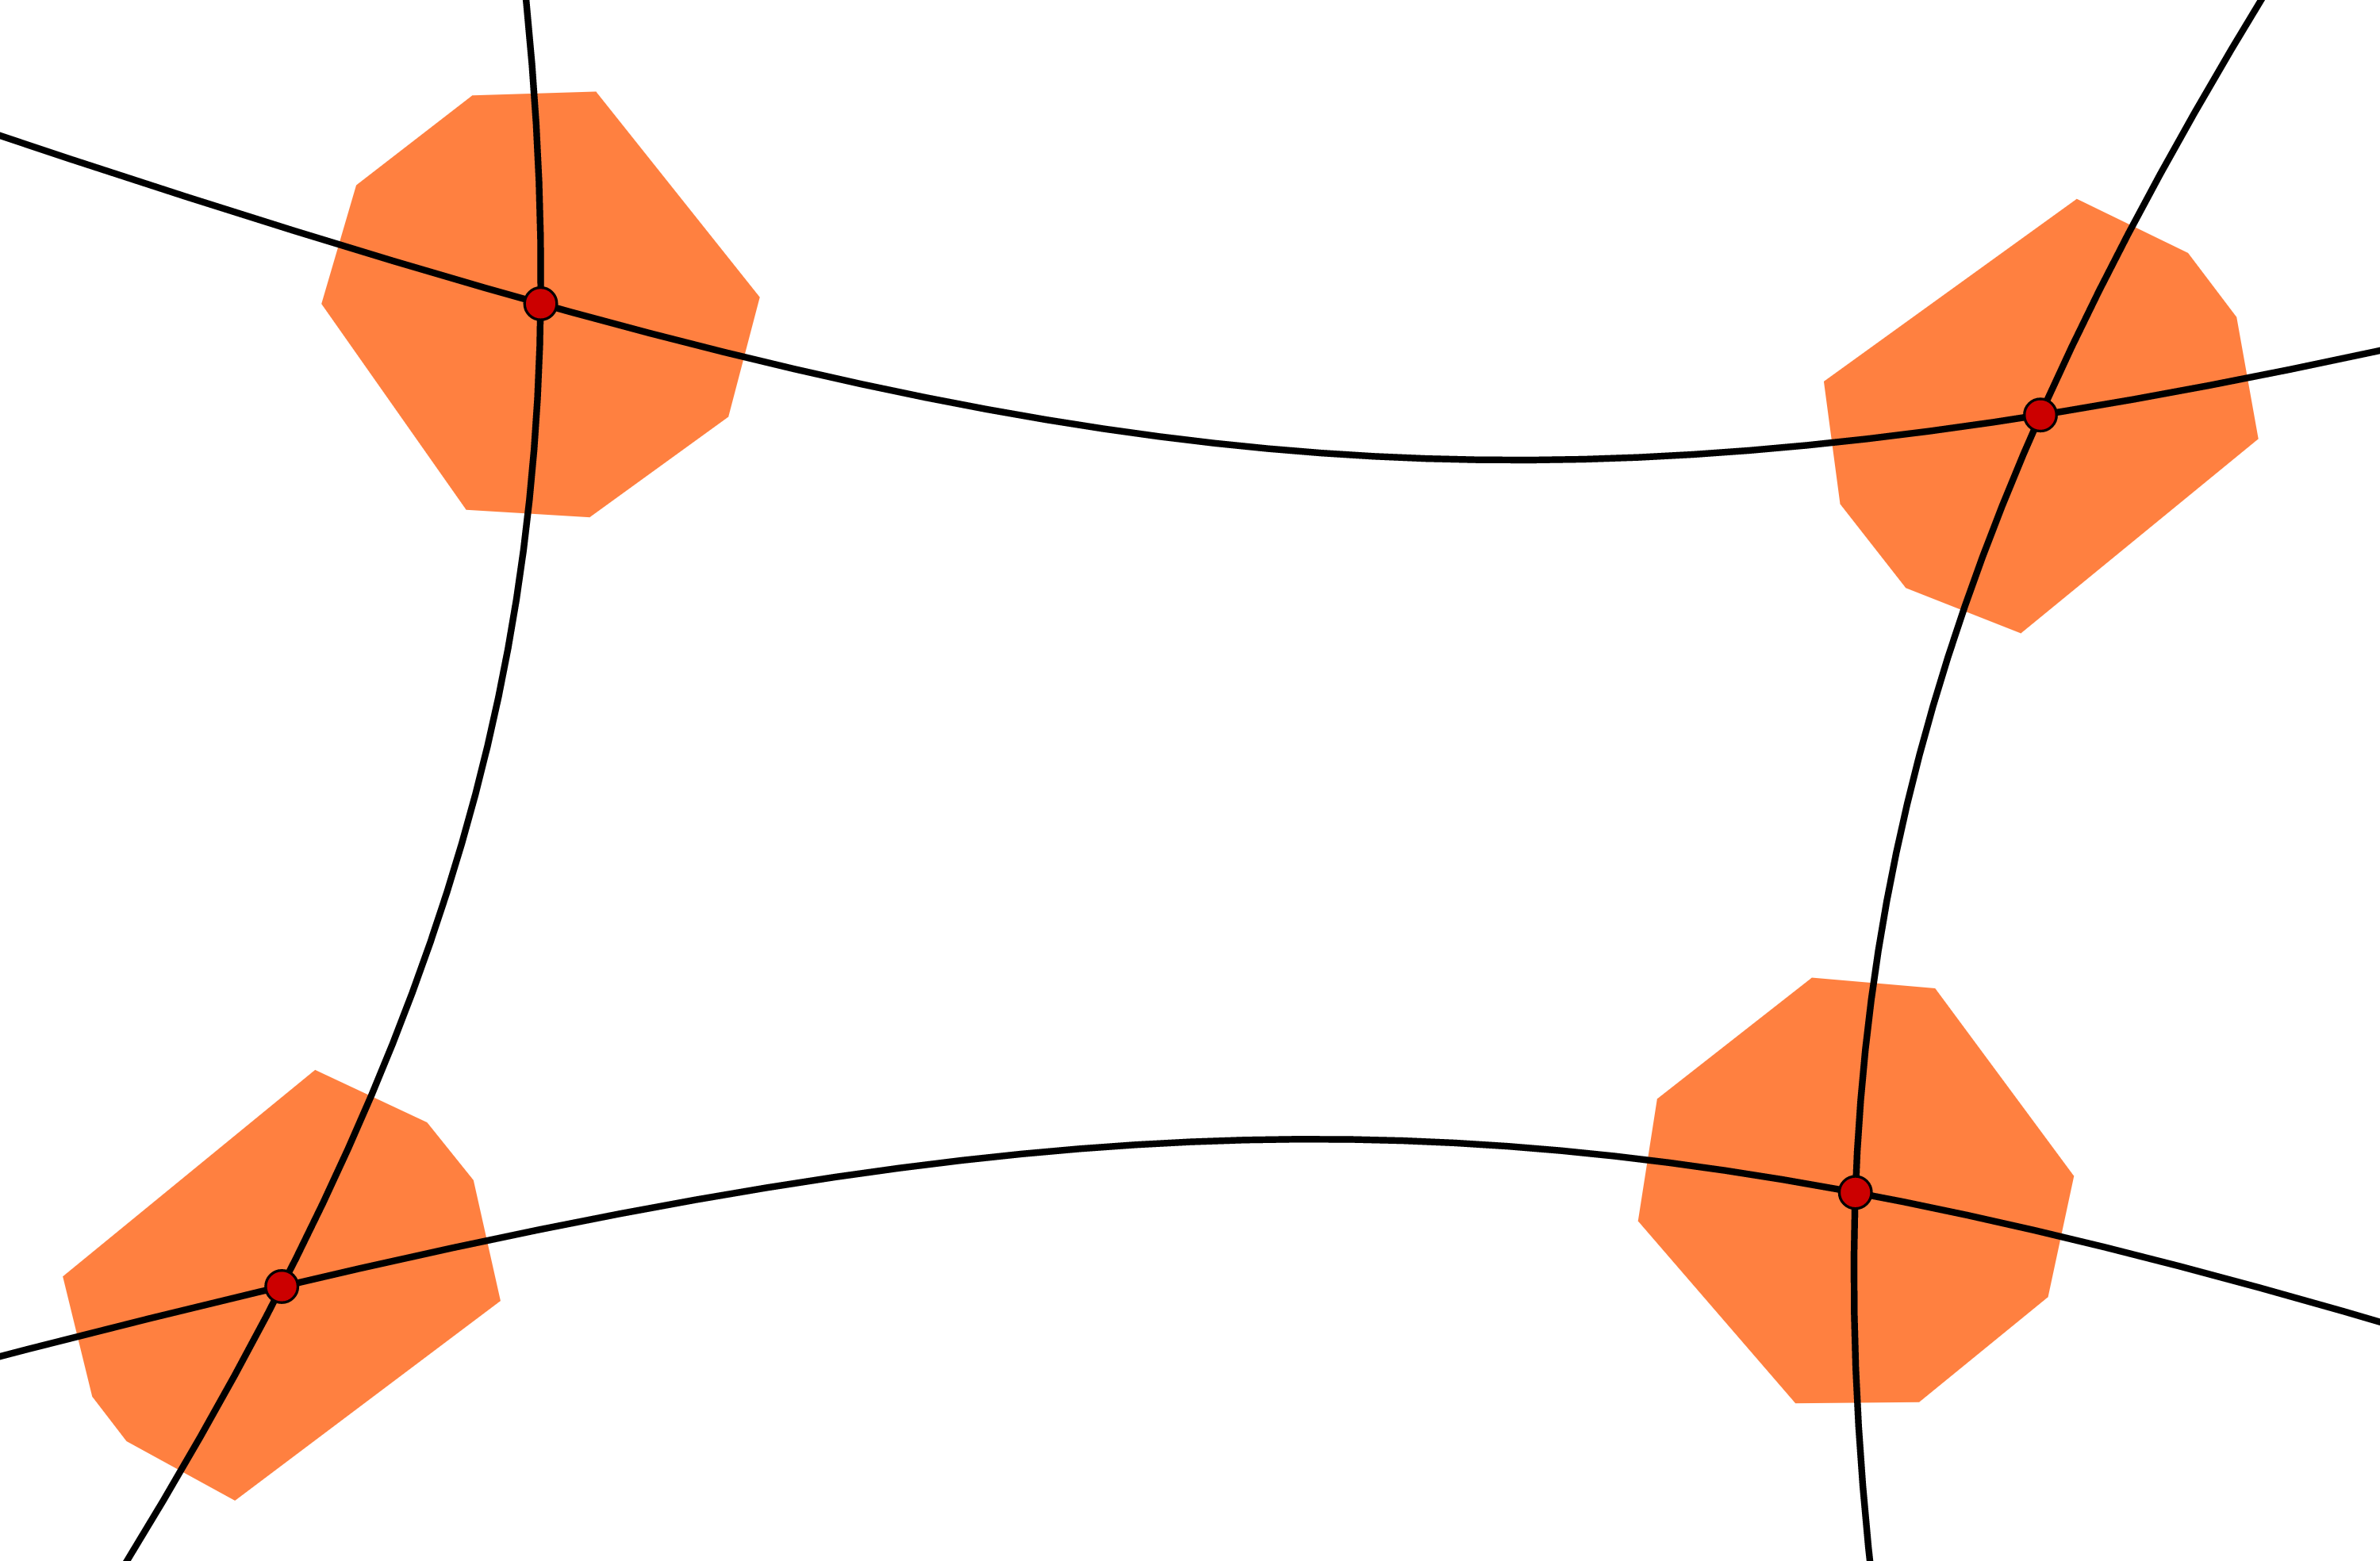
\includegraphics[width=0.5\textwidth]{figures/vertex-sleeve.png}
	\caption{
		\textbf{Forming vertex regions.}
		Octagonal sleeves are fit around codimension 2 singular values to form vertex regions.
		Codimension 1 singular values are illustrated in black and their crossings, codimension 2 singular values, are indicated in red.
		Note that the edges of the octagonal sleeves alternate between containing exactly one singular value, its intersection with a black arc, or consisting entirely of regular values.
	}
	\label{fig:vertex-sleeve}
\end{figure}

We begin by fitting octagonal sleeves around codimension 2 singular values as in Figure \ref{fig:vertex-sleeve}.
%Octagons are used here solely to simplify descriptions further down the line of proof.
Let $x$ be a codimension 2 singular value.
$x$ is the result of an arc crossing, and a small neighbourhood around an arc crossing is divided into four regions of regular values.
The octagon around $x$ is fit so its edges alternate between being fully contained in a region of regular values and orthogonally intersecting one of the arcs of singular values that creates $x$.
See Figure \ref{fig:vertex-sleeve} for a model fitting.

The interiors of the octagons along with the octagonal boundaries form the vertex regions of the stratification of $\RR$.
The octagons are chosen to be small enough that no two vertex regions overlap and such that the octagonal edges that intersect arcs of codimension 1 singular values are all the same length.

\begin{figure}[h!]
	\centering
	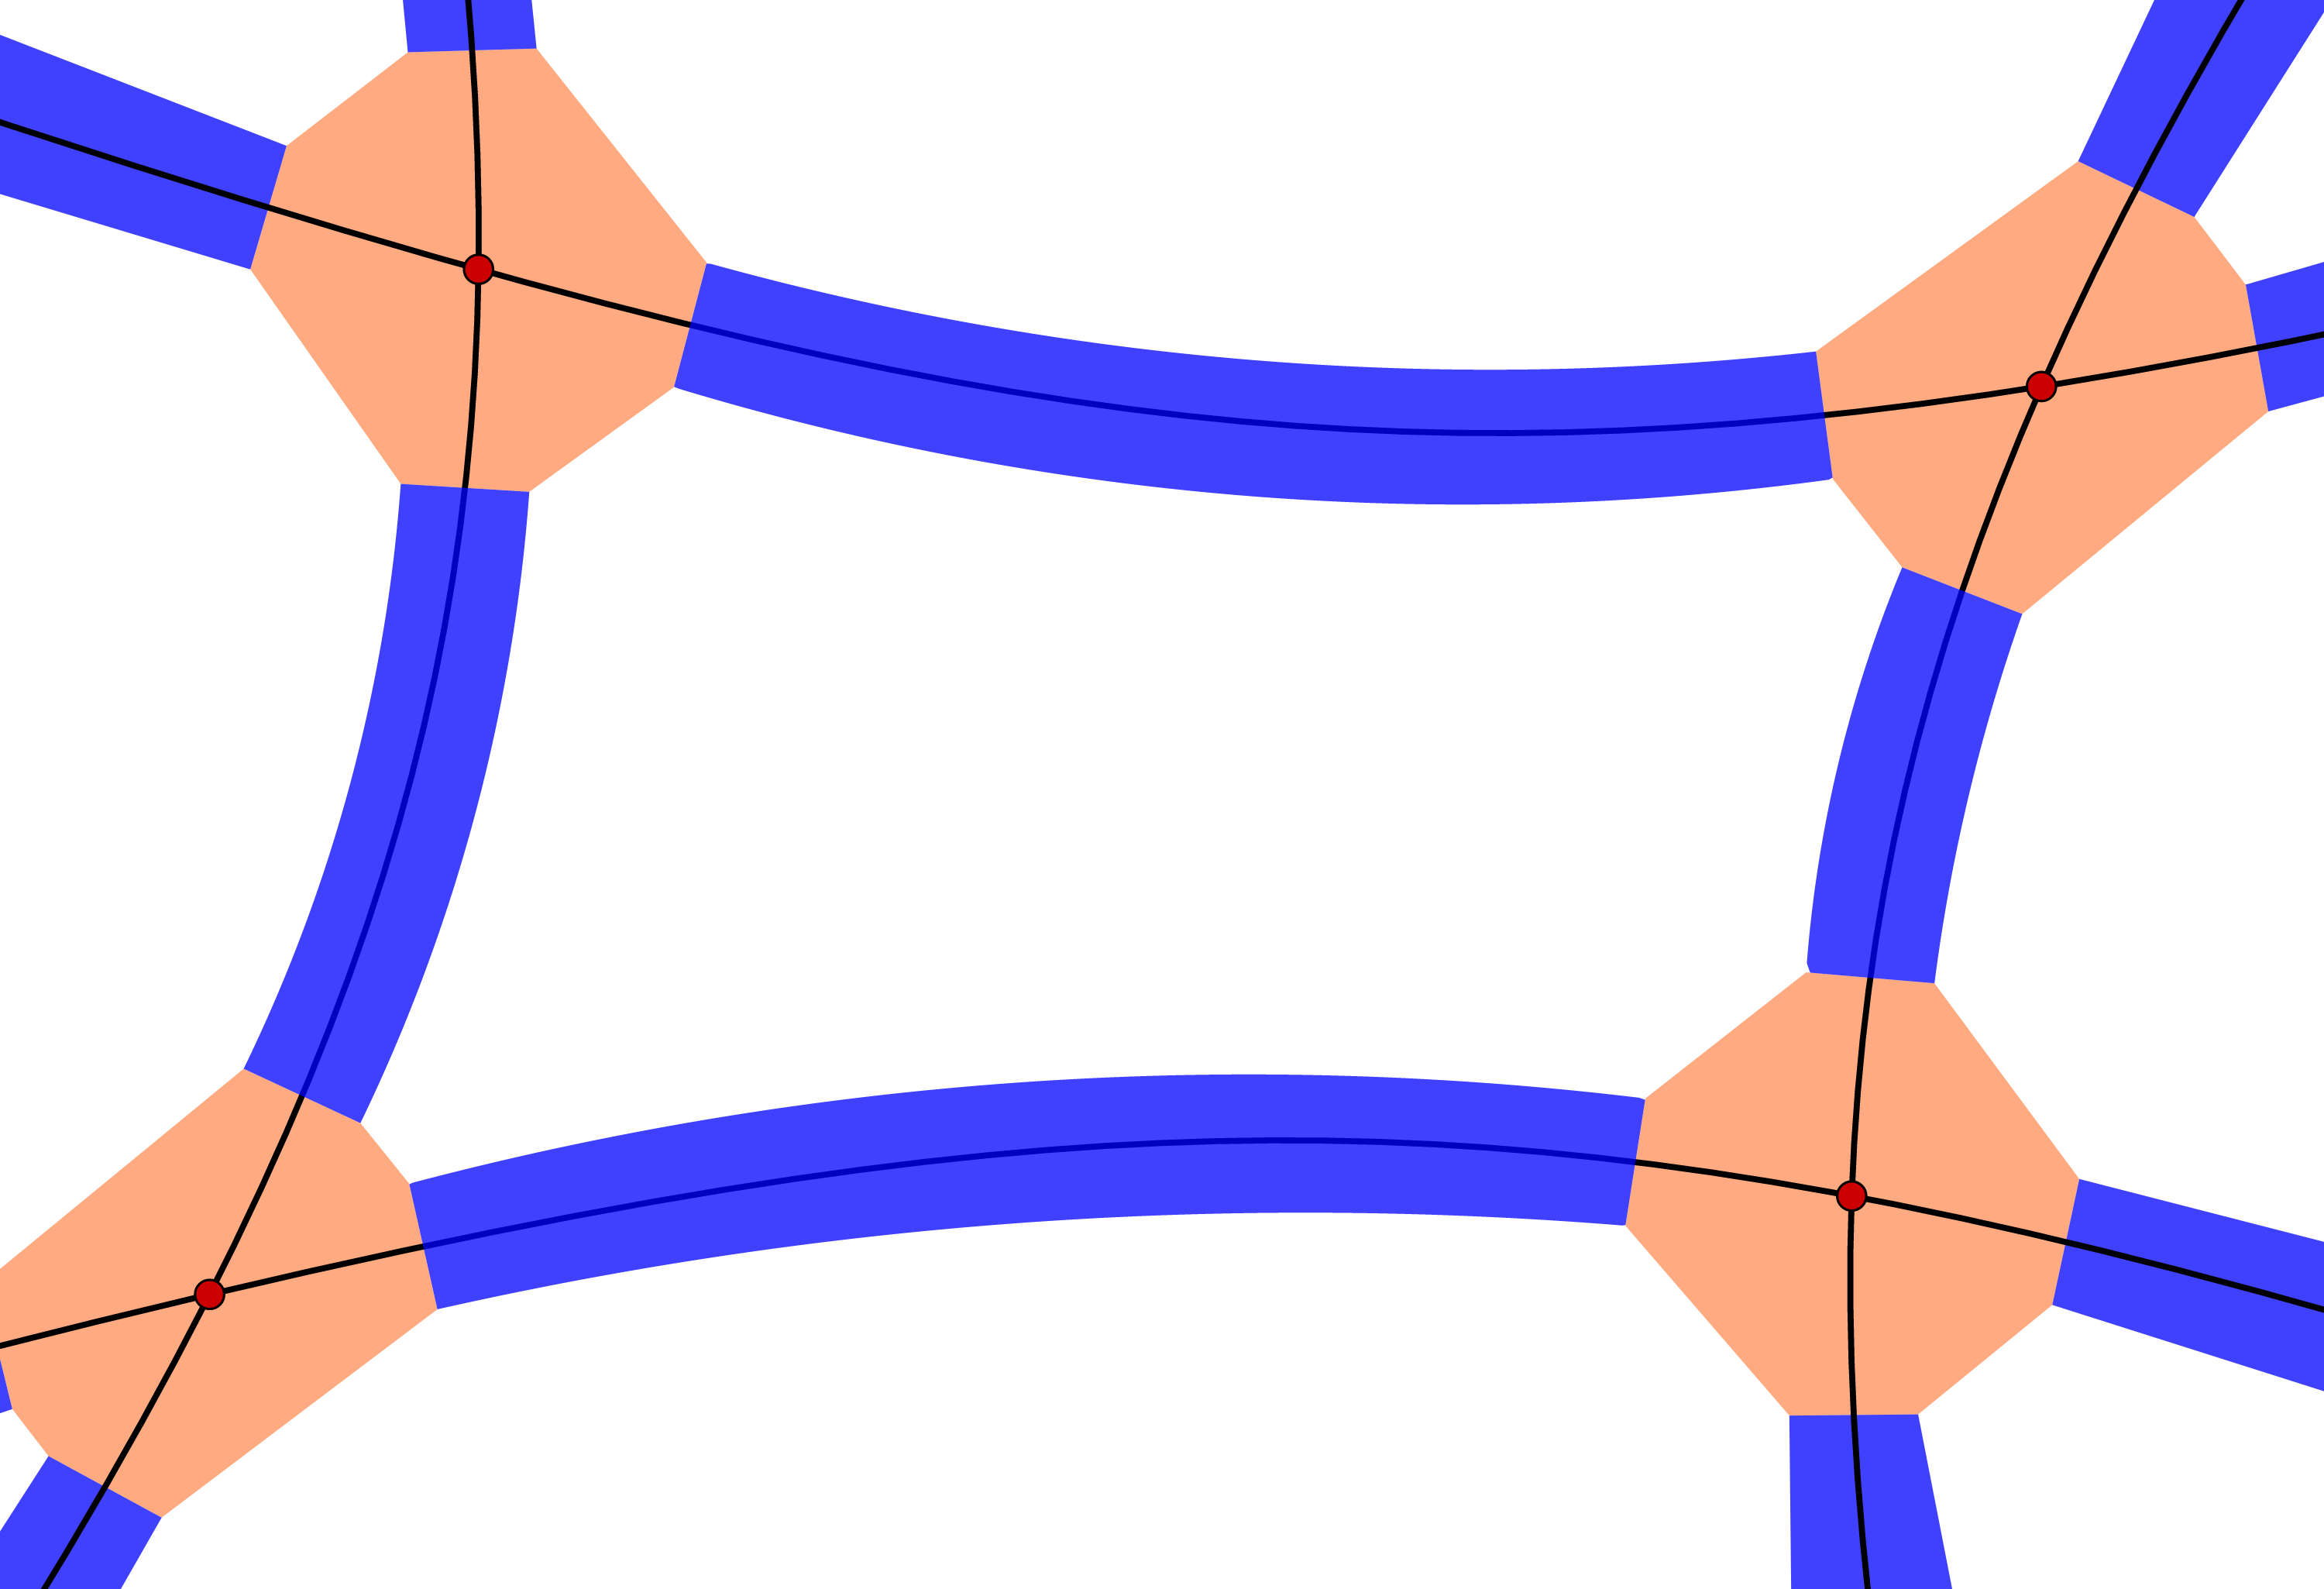
\includegraphics[width=\textwidth]{figures/edge-sleeve.png}
	\caption{
		\textbf{Forming edge regions.}
		Vertex region corners are connected to fit sleeves around arcs of codimension 1 singular values to form edge regions.  
	}
	\label{fig:edge-sleeve}
\end{figure}

Let $\gamma$ be an arc of codimension 1 singular values with endpoints a pair of codimension 2 singular values.
$\gamma$ orthogonally intersects one edge from each of the octagonal vertex regions fit around its endpoints, and we use these edges to form the edge region associated to $\gamma$ by connecting the endpoints of these edges to one another using a pair of arcs parallel to $\gamma$.
See Figure \ref{fig:edge-sleeve} for a model fitting.

The closures of the interiors of the shapes formed by the arcs and octagon edges form the edge regions of the stratification of $\RR$.
The octagonal edge endpoints are also vertices of the octagons, and the formation of edge regions uses every octagonal vertex as the endpoint of exactly one arc.

\begin{figure}[h!]
	\centering
	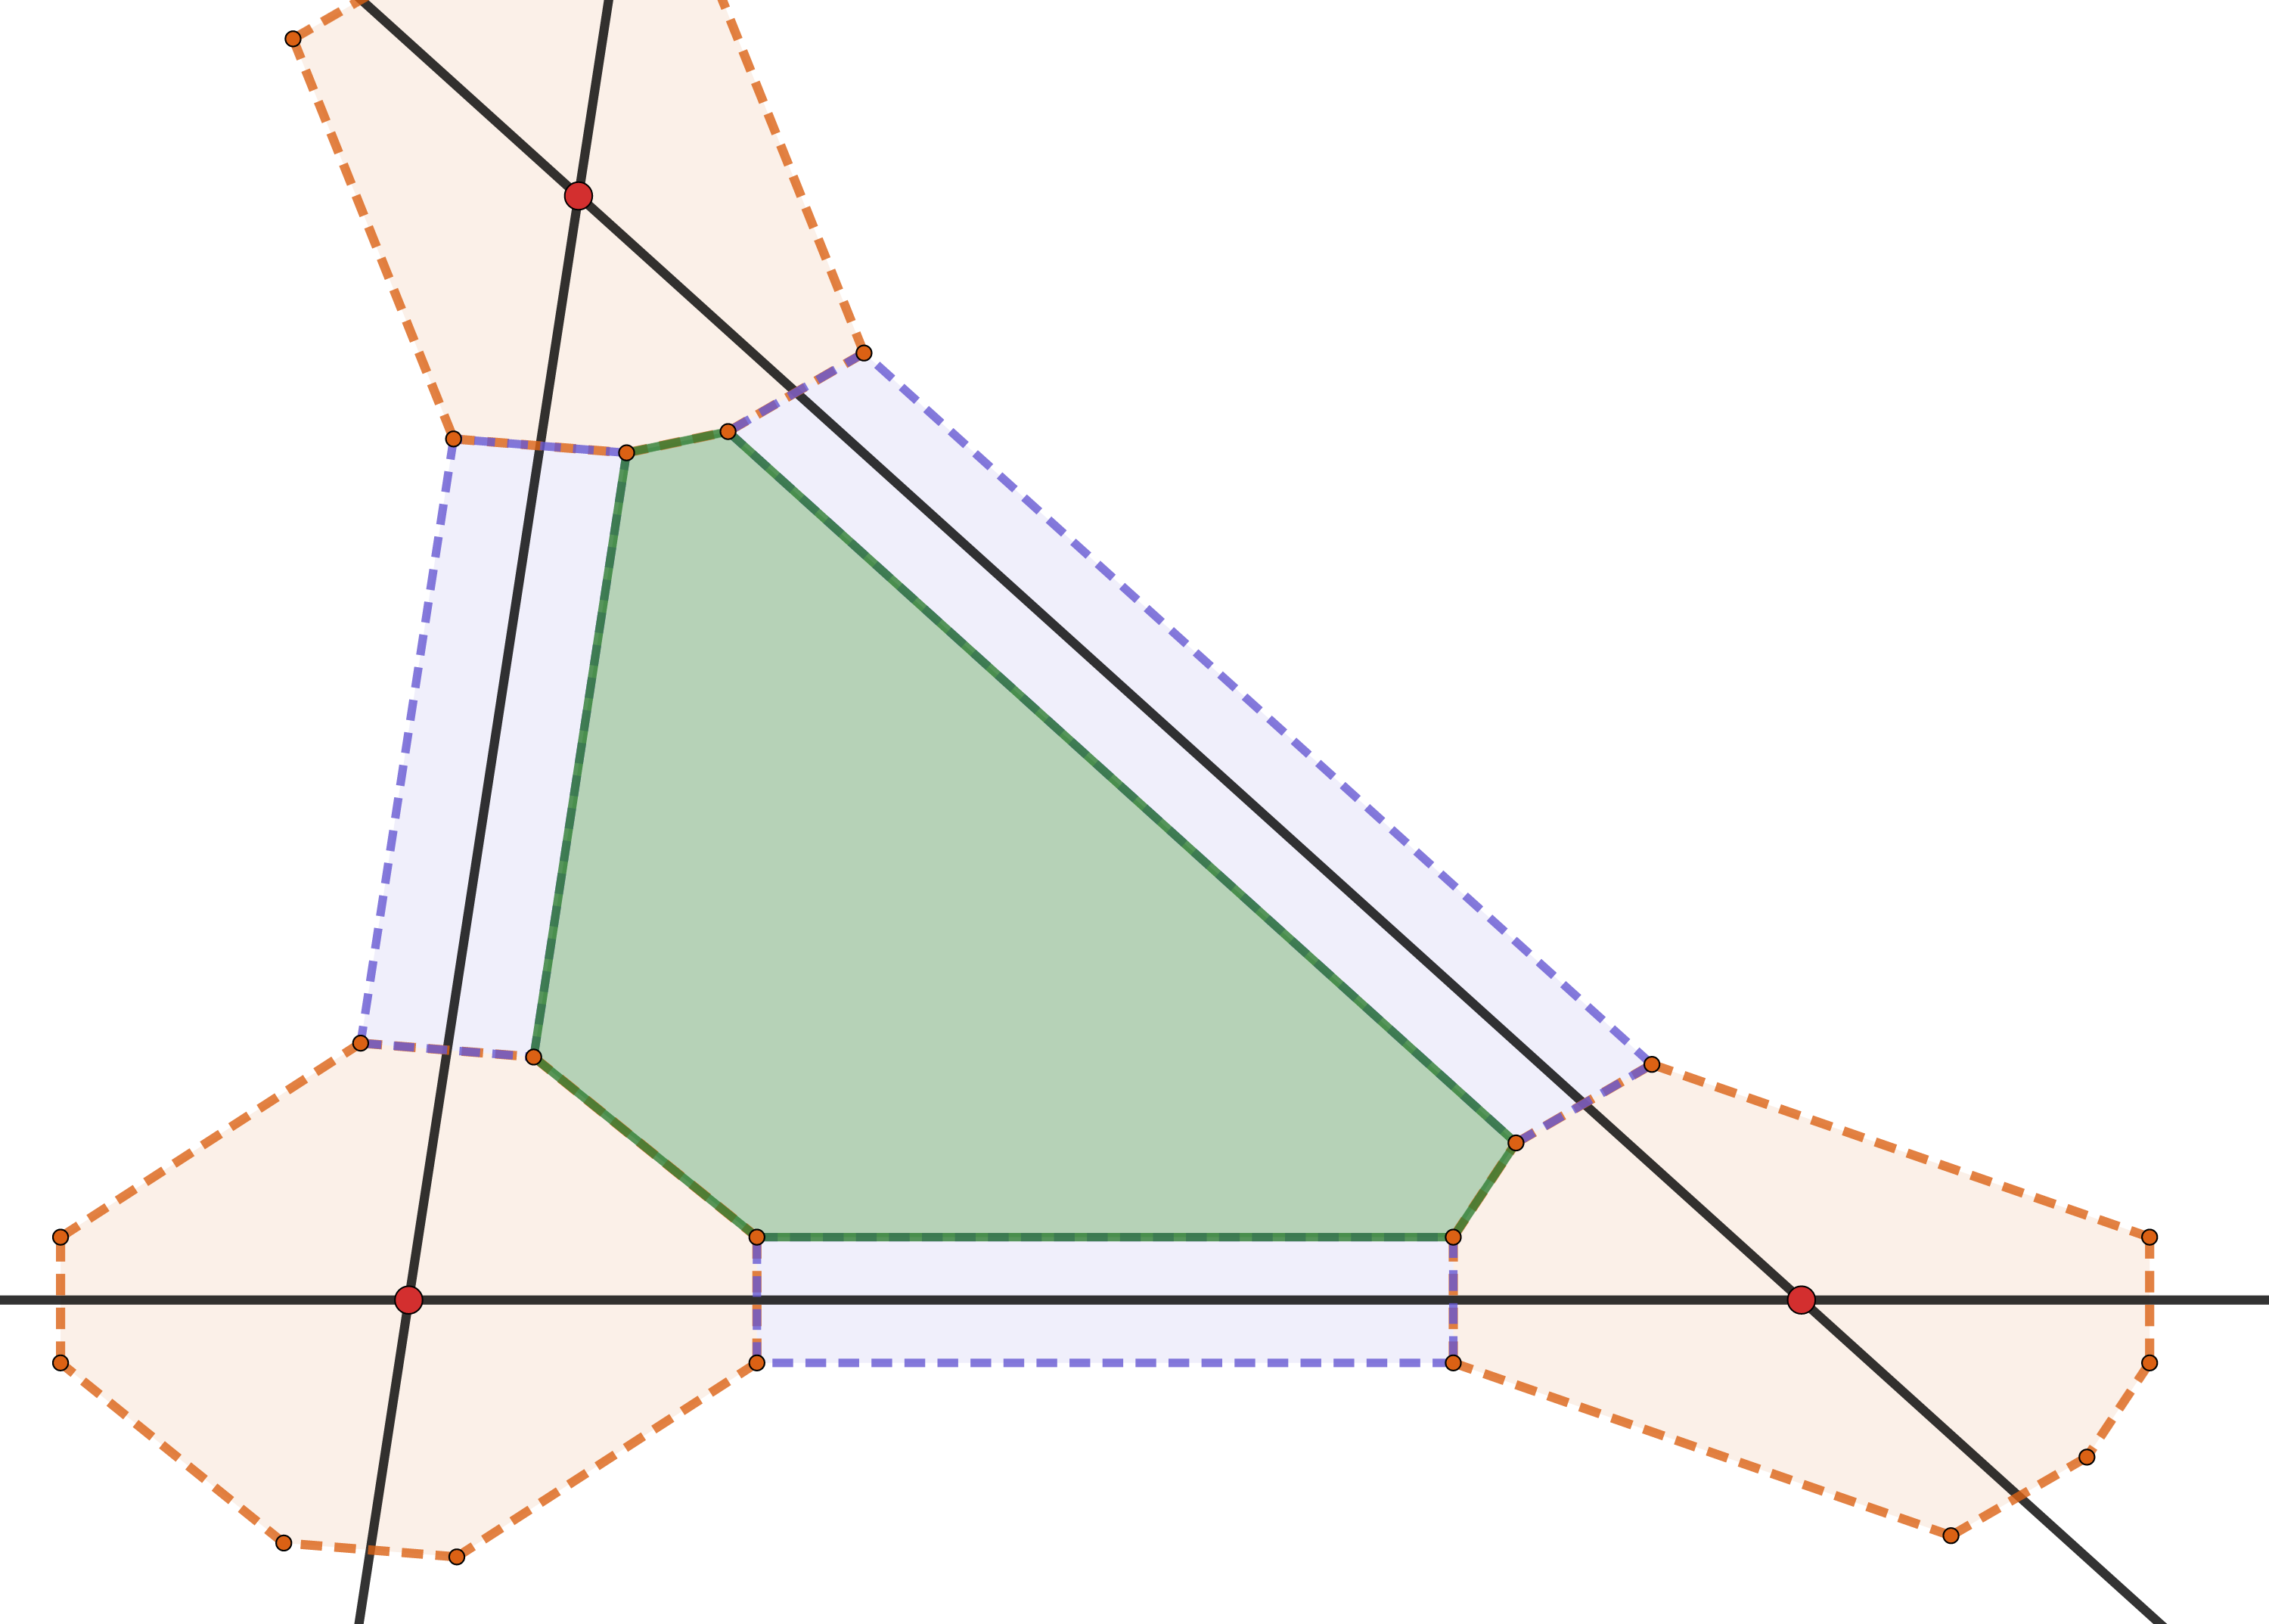
\includegraphics[width=\textwidth]{figures/face-sleeve.png}
	\caption{
		\textbf{Forming face regions.}
		All remaining regions contain no singular values, and we take these to be the face regions.
	}
	\label{fig:face-sleeve}
\end{figure}

Removing from $f(M)$ all vertex and edge regions, we are left with a collection of simply connected regions in the plane, each of which consists entirely of regular values.
We take the closures of these to be the face regions of the stratification of $\RR$.
The boundary of each face region is an alternating collection of arcs from edge regions and octagonal edges from vertex regions.
See Figure \ref{fig:face-sleeve} for a model fitting.

With all of the regions defined, we can describe precisely how $f$ stratifies $\RR$.
The stratification of $\RR$ is a stratification into subsets $R_{(i,j)}$ where $i,j$ are integers.
Subset indexing is defined so that a subset $R_{(i,j)}$ is an $i$--dimensional submanifold of $\RR$, thus $R_{(i,j)}\nleq R_{(k,l)}$ if $i\nleq k$.
The first collection of subsets used to filter $\RR$ are the corners of the octagonal vertex sleeves.
We assign to these subsets the indices $(0,i)$ for $i=1\dots N_0$, where $N_0$ is the number of corners.
Corners are disjoint, hence $R_{(0,i)}$ is not contained in $R_{(0,j)}$ for any $i, j$, whence $(0,i)\nleq (0,j)$ for any $i,j$.

The boundary arcs connect the $(0,i)$--level strata.
Arcs are indexed by $(1,j)$ for $j=1\dots N_1$, where $N_1$ is the number of arcs.
The boundary points of an arc are corners and are subsets of the filtration indexed by the $(0,i)$ indices, so $(0,i)\leq (1,j)$ if and only if $R_{(0,i)}$ is one of the boundary points of $R_{(1,j)}$.
Arcs intersect only at their boundary points, so $(1,j)\nleq(1,k)$ for any $j,k$. 

The regions themselves are indexed by $(2,k)$ for $k=1\dots N_2$, where $N_2$ is the number of regions.
These indices work similarly to the arc indices.
The boundary of a region consists of corners and arcs, so $(n,i)\leq(2,k)$ if and only if $R_{(n,i)}$ is contained in the boundary of $R_{(2,k)}$.

With $\RR$ stratified, we move onto a stratification of $M$.
This stratification is induced by the preimages of the strata of $\RR$.

%
%Before moving on to the stratification of $M$ induced by our decomposition of $\RR$, we need to iron out the corner cases of when $X_f$ contains no codimension 2 singular values.
%
%
%Because $X_f$ is connected, $X_f=f(S_1(f))$, and $S_1(f)$ is a collection of smooth non-intersecting curves in $M$, we conclude that $S_1(f)$ contains exactly one curve.
%Furthermore, $f(M\setminus S_1(f))$ lies entirely within $X_f$ so $S_1(f)$ is everywhere a definite fold.
%
%...



\section{Stratifying $M$}

Decomposing $\RR$ via the singular values of $f$ also induces a stratification of $M$ by considering the preimage through $f$ of the decomposing regions.
The interiors of a face regions have preimage through $f$ a disjoint collection of face blocks, the interiors of edge regions have preimage of edge blocks, and of vertex regions, vertex blocks.

To understand the structure of face, edge, and vertex blocks we investigate the preimages of regular and singular values of $f$ in the plane.
\begin{defn}
	Because $M$ is closed, $f$ is proper.
	Thus, for any point $q$ in $f(M)$, a fiber of $f$ above $q$ (i.e.\ a connected component of $f\inv(q)$) is either a closed 1--manifold (i.e.\ $S^1$) or contains a critical point of $f$.
	
	We define a \emph{singular fiber} to be a fiber that contains a critical point of $f$, and a \emph{regular fiber} to be a fiber consisting entirely of regular points.	
\end{defn}


\section{Attach Handles}

Stratifying $M$ allows the definition of attachment neighbourhoods for stratified 2--, 3--, and 4--handles in $W=M\times\Ilit$.
A 4--dimensional 2--handle is attached over a closed solid torus embedded in the boundary of a 4--manifold, so attachment neighbourhoods for our stratified 2--handles are straightforward: they are the face blocks of $M$.
We alter the boundary of $W$ by attaching handles, so the attachment neighbourhoods for 3--handles (4--handles, resp.) must be found after 2--handles (3--handles, resp.) are attached.
For a 3--handle, an attachment neighbourhood consists of the union of an edge block with some strata introduced by 2--handle attachment.
For a 4--handles, an attachment neighbourhood consists of the union of an edge block with some strata introduced by 2-- and 3--handle attachment.
We investigate the consequences of handle attachment by comparing the boundary of the initial manifold with the boundary of the manifold resulting from handle attachment, and use a precisely defined handle structure to focus the investigation.
Our first step is to precisely define the structure of the stratified 2--handles that we are attaching.

\subsection{2--handles}

Let $B$ be a face block of $M_1$.
By Theorem \ref{thm:block-structure}, $B$ is a closed solid torus that is stratified-homeomorphic to $S^1\times G_n$, where $G_n$ is an $n$--gon for some $n$.
Consider an unknotted embedding of $B$ in $S^3$, as illustrated in Figure \ref{fig:face-block-complement}.
The complement of the interior of $B$ is another closed solid torus $B'$, and we stratify $B'$ as follows.
First include the shared stratified boundary of $B$.
Next, introduce meridinal disks of $B'$ that are bounded by the $(1,i)$--indexed strata in $B$, i.e.\ the boundary curves in $B$ corresponding to $S^1\times c_m$ where $c_m$ is a corner of $G_n$, $m=1\dots n$.
Finally, add the homeomorphic 3--disks of $B'$ whose boundaries consist of one longitudinal annulus of $B$ along with the two meridinal disks in $B'$ that are bounded by the annulus's circular boundary components.
The filtration of $B'$ is created identically to that of the original face blocks, using inclusion as a partial ordering and indexing a stratum by its dimension as a submanifold of $B'$.
Figure \ref{fig:face-block-complement} illustrates a face block $B$ and its complement inside of $S^3$.

\begin{figure}[h!]
	\centering
	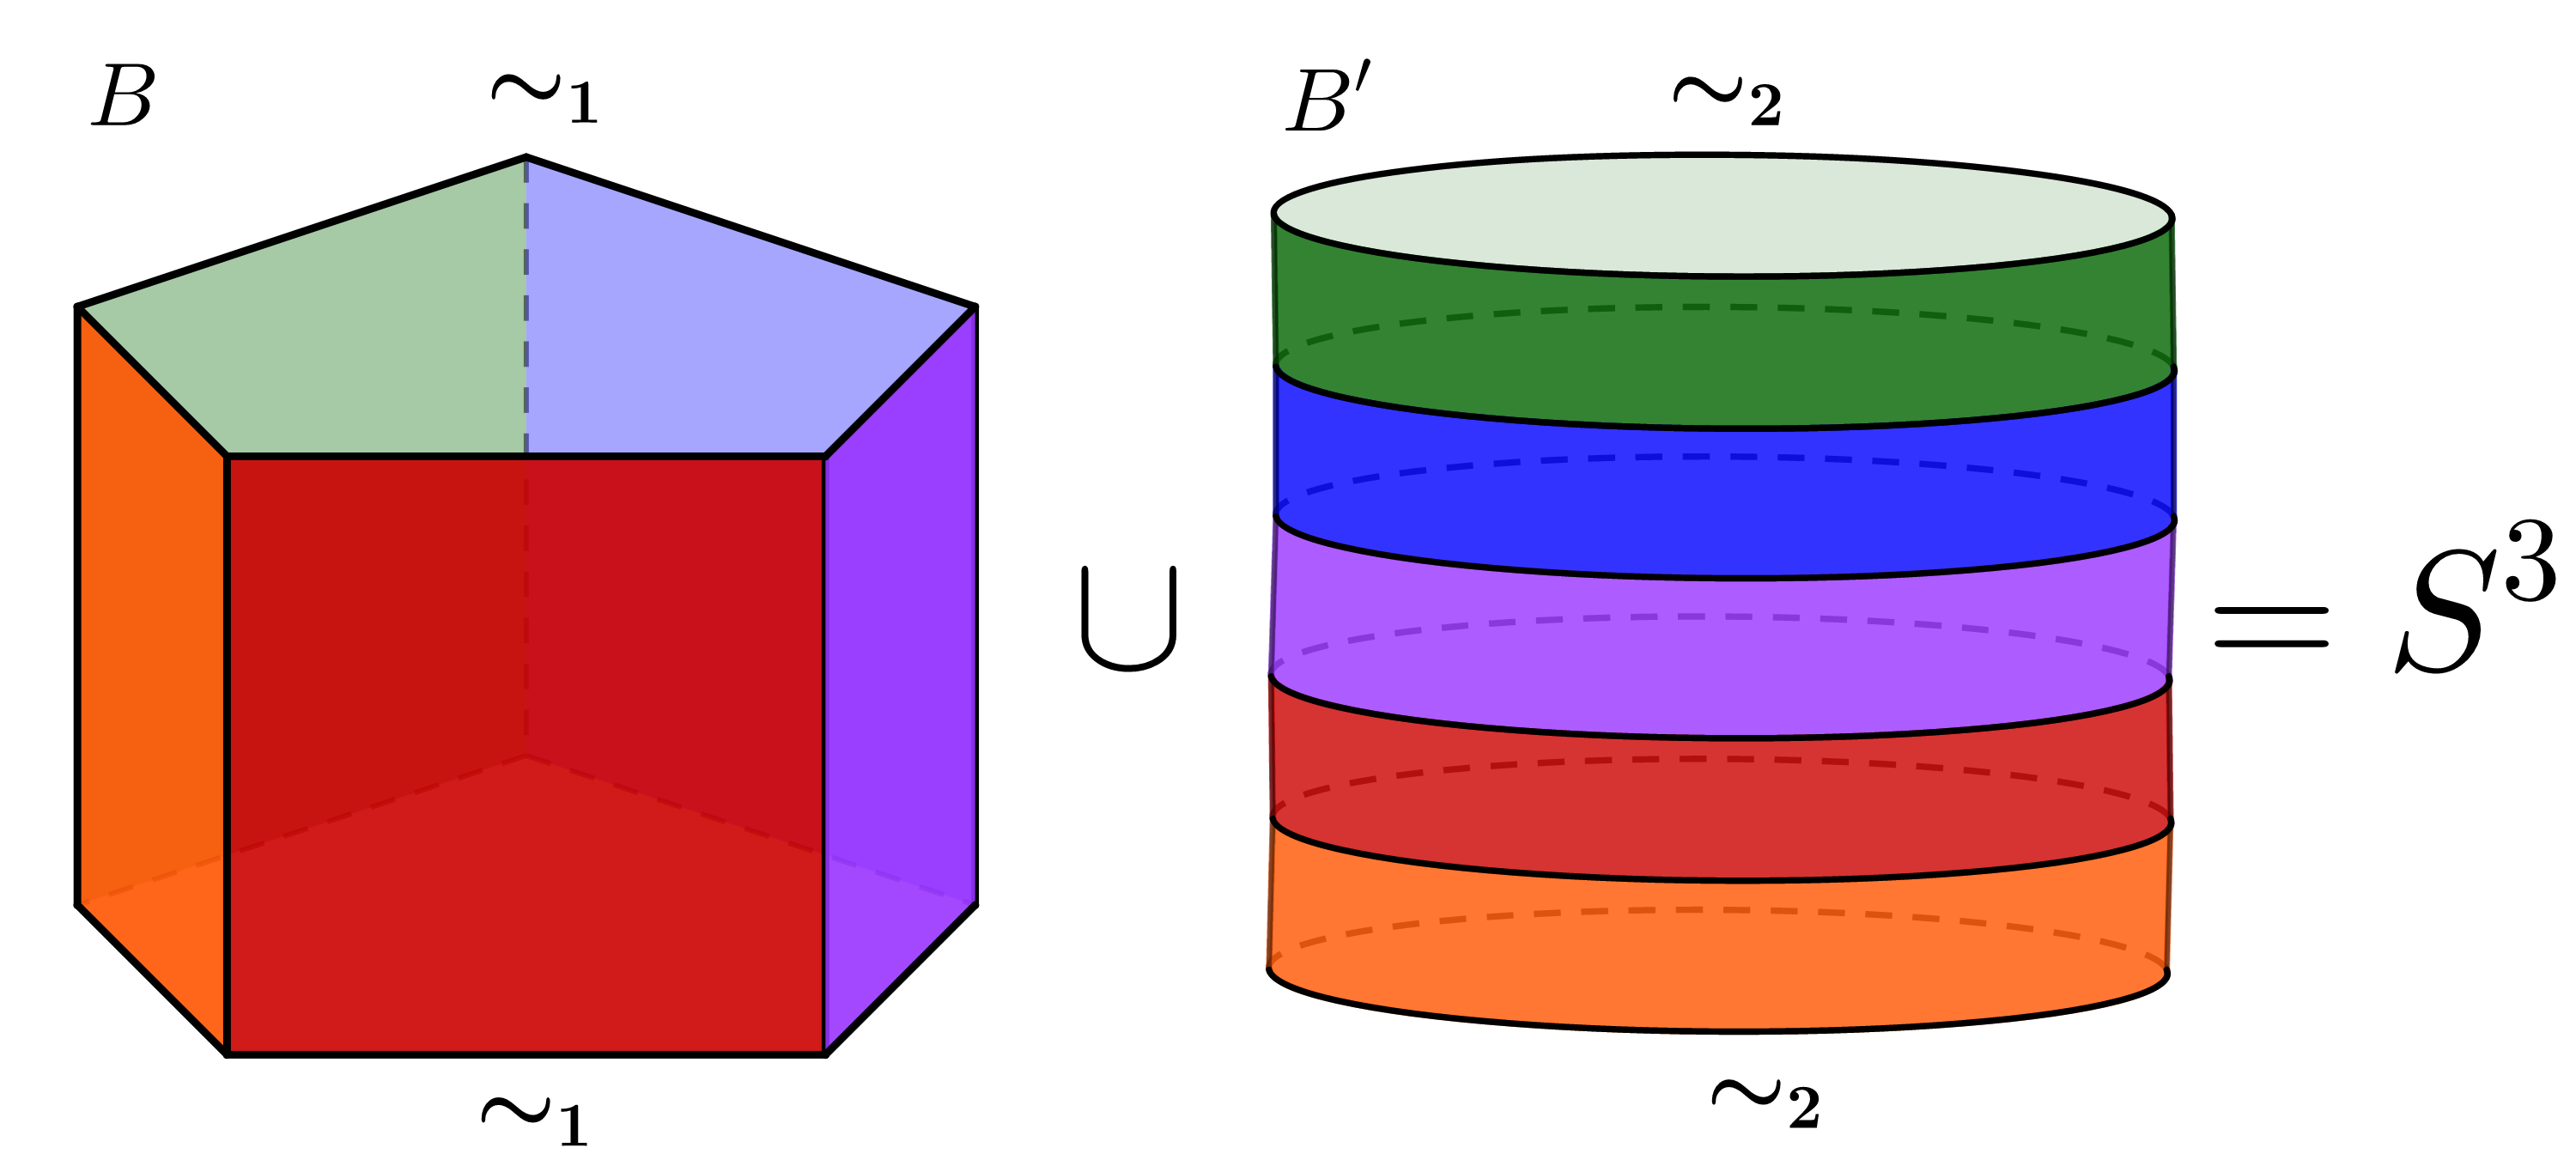
\includegraphics[width=\textwidth]{figures/face-block-complement.png}
	\caption{
		\textbf{A face block and its complement form $S^3$.}
		A face block $B$ is a stratified closed solid torus that is stratified-homeomorphic to $S^1\times G_n$ for some $n$--gon $G_n$.
		The complement of its unknotted interior in $S^3$ is another stratified closed solid torus $B'$.
	}
	\label{fig:face-block-complement}
\end{figure}

Taking $S_B^3$ to be the stratified $S^3$ formed as the union of $B$ and $B'$, we craft a stratified 2--handle structure as $C(S_B^3)$, the cone of $S_B^3$.
We call $C(S_B^3)$ the \emph{stratified 2--handle induced by $B$}.
Attaching $C(S_B^3)$ to $W$ over $B\subset M_1$ alters the boundary of $W$ by replacing $B\subset M_1$ with $B'$.
The full extent of this surgery can be detected by examining the edge and vertex blocks of the stratification that are incident to $B$.

\begin{theorem}
	\label{thm:primed-block-structure}
	Let $M$ be a smooth, closed, stratified, orientable 3--manifold with stratification induced by a stratifying map $f$, let $\mathfrak{B}$ be the set of face blocks of $M_1$, and let $W=M\times\Ilit$.
	Consider the 4--manifold $W'$ constructed from $W$ as
	\[
		W' = W\cup\{C(S_B^3)\}_{B\in \mathfrak{B}} / \sim,
	\]
	where $\sim$ is defined by $b\sim \iota(b)$, $\iota$ the identity map $C(S_B^3)\supset B\overset{\iota}{\to} B\subset M_1$.
	Then $M_1'=\pd W'\setminus M_0$ is a stratified 3--manifold with a decomposition into \emph{primed edge blocks} and \emph{primed vertex blocks} such that the decomposition is well-defined and the primed blocks have the following structure:
	\begin{itemize}
		\item \emph{primed edge block:}
		Let $E'$ be a primed edge block.
		Then $E'$ is identical to an edge block $E$ from Theorem \ref{thm:block-structure} with cylinders (copies of $D^2\times\Ilit$) glued over all annular boundary strata of $E$ (i.e. each closed strata $A$ of $E$ such that $A=E\cap B$ for some face block $B\in\mathfrak{B}$).
		Thus $E'$ is a stratified 3--manifold homeomorphic to $S^2\times\Ilit$
		
		\item \emph{primed vertex block:}
		Let $V$ be a primed vertex block.
		Then $V$ is identical to a vertex block from Theorem \ref{thm:block-structure} with cylinders glued over each annular boundary stratum $A$ of $V$ such that $A=V\cap B$ for some face block $B\in\mathfrak{B}$.
		Thus $V$ is a stratified 3--manifold whose boundary components are each homeomorphic to $S^2$.
	\end{itemize}
\end{theorem}

\begin{proof}
	We split the proof of this theorem into three parts.
	In the first two parts, we prove that we can find the prescribed primed edge and vertex block structures in $M_1'$.
	In the third part, we show that these structures exhaust $M_1'$.
	
	\textbf{Part 1:}
	Edge blocks occur in three possible forms: regular edge blocks as $A\times\Ilit$, definite edge blocks as $D^2\times\Ilit$, and indefinite edge blocks as $P\times\Ilit$.
	Figure \ref{fig:edge-block-incidence} displays the possible edge block forms and indicates the boundary strata of an edge block that are shared by face blocks.
	
	\begin{figure}[h!]
		\centering
		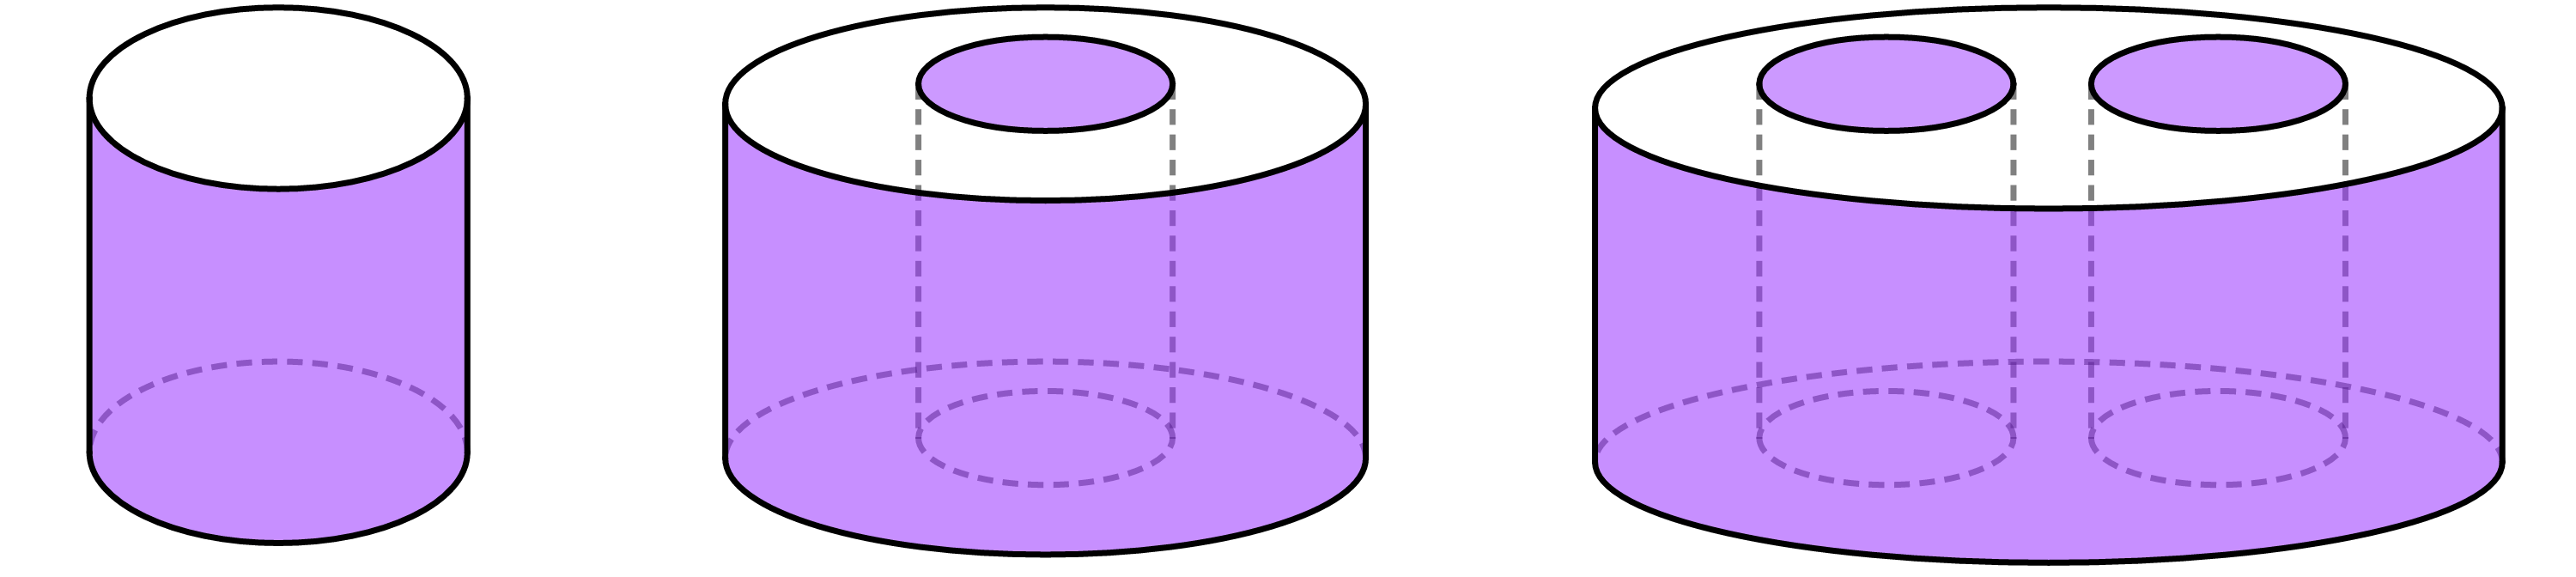
\includegraphics[width=\textwidth]{figures/edge-block-incidence.png}
		\caption{
			\textbf{Edge blocks.}
			The possible edge blocks of $M_1$.
			Annular boundary strata that are incident with face blocks of $M_1$ are indicated in purple.
			For each block, gluing cylinders over the indicated annuli results in a stratified 3--manifold homeomorphic to $S^2\times\Ilit$.
		}
		\label{fig:edge-block-incidence}
	\end{figure}
	
	Figure \ref{fig:edge-face-shared-boundary} shows the annulus shared by a model edge block $E$ and $B$ in $M_1$ and its corresponding annulus shared by $B$ and $B'$ in $S_B^3$.
	The figure demonstrates that the effect on $\pd W$ near $E$ of attaching $C(S_B^3)$ over $B$ is equivalent to gluing a well-defined cylinder from the stratification of $B'$  to $E$ over the annular boundary stratum $E\cap B$.
	Attachment of all 2--handles applies this cylinder gluing to all annular strata of $E$, and applying this cylinder gluing to all annular strata of $E$ results in a 3--manifold homeomorphic to $S^2\times\Ilit$.

	\begin{figure}[h!]
		\centering
		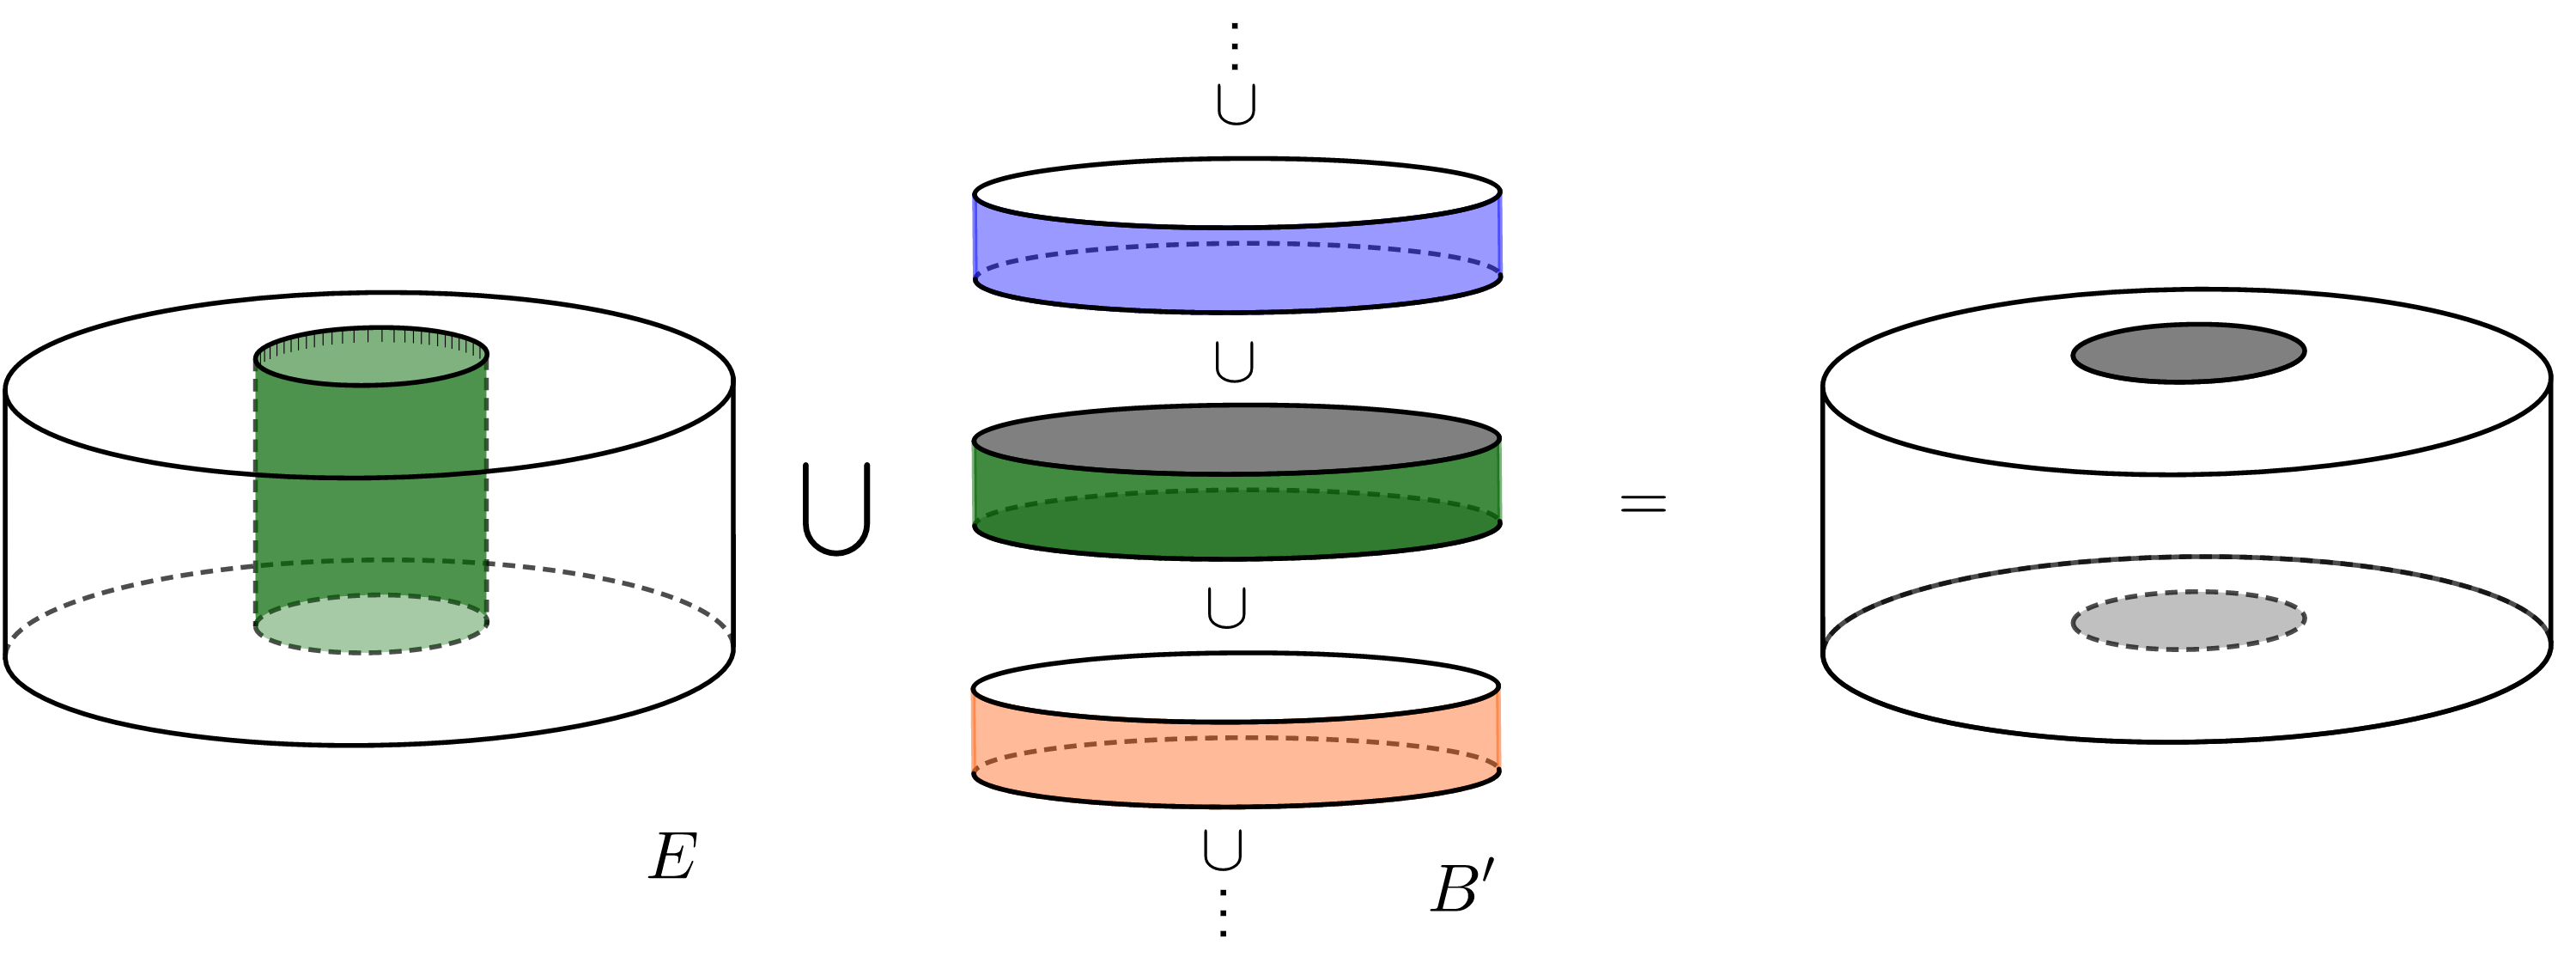
\includegraphics[width=\textwidth]{figures/edge-face-shared-boundary.png}
		\caption{
			\textbf{The effect of stratified 2--handle attachment on a model edge block.}
			A model edge block $E$, a face block complement $B'$, and the result of attaching $C(S_B^3)$ to $W$ over $B$ on $E$.
			The boundary stratum shared by $E$ and $B$ in $M_1$ is indicated in green, as is the corresponding boundary stratum of $B'$ in $S_B^3$.
		}
		\label{fig:edge-face-shared-boundary}
	\end{figure}
	
	\textbf{Part 2:}	
	Vertex blocks occur in five possible forms: regular vertex blocks as $S^1$-bundles over the vertex region, indefinite and definite vertex blocks stratified-homeomorphic to those that appear in Figure \ref{fig:codim-1-blocks}, and interactive vertex blocks stratified-homeomorphic to the handlebodies in Figures \ref{fig:codim-2-surface-1} and \ref{fig:codim-2-surface-2}.
	Figure \ref{fig:vertex-block-incidence} displays the possible vertex block forms embedded in $S^3$ and indicates the boundary strata of a vertex block that are shared by face blocks.
	
	\begin{figure}[h!]
		\caption{
			\textbf{Vertex blocks.}
			The possible vertex blocks of $M_1$.
			Annular boundary strata that are incident with face blocks of $M_1$ have been indicated.
			Gluing cylinders over the indicated annuli results in a stratified 3--manifold whose boundary is a collection of stratified 2--spheres.
		}
		\label{fig:vertex-block-incidence}
	\end{figure}	
	
	Figure \ref{fig:vertex-face-shared-boundary} displays a model vertex block $V$ embedded on the `outside' of its stratified genus-3 boundary surface in $S^3$, and shows the annulus shared by $V$ and $B$ in $M_1$ and its corresponding annulus shared by $B$ and $B'$ in $S_B^3$.
	The figure demonstrates that the effect on $\pd W$ near $V$ of attaching $C(S_B^3)$ over $B$ is equivalent to gluing a well-defined cylinder from the stratification of $B'$  to $V$ over the annular boundary stratum $V\cap B$.
	Attachment of all 2--handles applies this cylinder gluing to all annular strata of $V$ shared by face blocks, and applying this cylinder gluing to such annular strata of $V$ results in a 3--manifold whose boundary components are each homeomorphic to $S^2$.
	Moreover, these boundary components are exactly the boundary components of the primed edge blocks.
	
	\begin{figure}[h!]
		\caption{
			\textbf{The effect of stratified 2--handle attachment on a model vertex block.}
			A model edge block $V$, a face block $B$, its complement $B'$, and the effect of attaching $C(S_B^3)$ to $W$ over $B$ on $V$.
			The boundary stratum shared by $V$ and $B$ in $M_1$ is indicated, as is the corresponding boundary stratum of $B'$ in $S_B^3$.
		}
		\label{fig:vertex-face-shared-boundary}
	\end{figure}

	\textbf{Part 3:}
	To show that primed edge and vertex blocks exhaust $M_1'$, we show that the entirety of $B'$ has been apportioned among the primed blocks for each $B'$.
	The $(3,k)$ strata of $B'$ are each cylinders whose annular boundary strata corresponds directly to a longitudinal boundary annulus of $B$.
	Such an annulus projects through $f$ to a boundary edge of a face region.
	Face regions do not intersect even on their boundary, so all of the annular boundary strata of $B$, hence $B'$, are shared only by edge and vertex blocks.
	Thus each cylinder of $B'$ has been assigned to a primed edge or vertex block.
	Because 2--handle attachment altered $M_1$ to $M_1'$ only by replacing each face block $B$ with its complementary $B'$, the primed blocks must exhaust $M_1'$.
\end{proof}

Decomposing $M_1'$ into primed edge and vertex blocks provides us with stratified 3--handle attachment neighbourhoods.
A 4--dimensional 3--handle is attached over an $S^2\times\Ilit$ embedded in the boundary of a 4--manifold, so attachment neighbourhoods for our stratified 3--handles are the primed edge blocks of $M_1'$.
We begin 3--handle attachment by precisely defining the structure of a stratified 3--handle so that it may be attached over a primed edge block.

\subsection{3--handles}
\label{subsec:smooth-3handles}

Let $E'$ be a primed edge block of $M_1'$.
By Theorem \ref{thm:primed-block-structure}, $E'$ is homeomorphic to $S^2\times\Ilit$.
In particular, $\pd E'$ is a disjoint pair of stratified 2--spheres.
We form a 4--disk containing $E'$ in its boundary by a double coning method on $E'$: we first cone the spherical boundary components of $E'$ to form a pair of 3--disks, glue these 3--disks to $E'$ to form a 3--sphere, then cone the 3--sphere to obtain a 4--disk.

For each stratified boundary sphere $S_i^2\in\pd E'$ we form the stratified 3--disk $C(S_i^2)$ and glue $C(S_i^2)$ to $E'$ over $S_i^2$.
The result is a stratified 3--sphere, and we further cone that 3--sphere to form a stratified 4--disk.
We denote the 4--disk by $C^2(E')$ and call the resulting stratified 3--handle structure the \emph{stratified 3--handle induced by $E'$}.
Attaching $C^2(E')$ to $W'$ over $E'\subset M_1'$ alters the boundary of $W'$ by replacing $E'$ with the 3--disks $C(S_i^2)$ glued over the corresponding stratified boundary spheres in $M_1'$.
The full extent of this surgery can be detected by examining the primed vertex blocks of $M_1'$.

\begin{cor}
	\label{thm:primed-primed-block-structure}
	Let $W'$ be the 4--manifold resulting from the construction described in Theorem \ref{thm:primed-block-structure} and let $\mathfrak{E}'$ be the set of primed edge blocks of $M_1'\subset\pd W'$.
	Consider the 4--manifold $W''$ constructed from $W'$ as
	\[
	W'' = W'\cup\{C^2(E')\}_{E'\in \mathfrak{E}'} / \sim,
	\]
	where $\sim$ is defined by $e\sim \iota(e)$, $\iota$ the identity map $C^2(E')\supset E'\overset{\iota}{\to} E'\subset M_1'$.
	Then $M_1''=\pd W''\setminus M_0$ is a stratified 3--manifold with a decomposition into \emph{double primed vertex blocks} $V''$ such that the decomposition is well-defined and each $V''$ is homeomorphic to $S^3$.
\end{cor}

\begin{proof}
	For each vertex block $V$, the cylinders introduced by 2--handle attachment and the 3--disks introduced by 3--handle attachment combine into a handlebody $H$ of the same genus as $V$.
	$V$ and $H$ combine to form each component of $M_1''$, and we show a Heegaard diagram of complementary meridinal circles for each case in Figures \ref{fig:heegaard-genus-0}-\ref{fig:heegaard-genus-3-2}.
	Thus $M_1''$ consists of a collection of stratified 3--spheres \cite{SchlWald}.
	
	\begin{figure}[h!]
		\caption{
			\textbf{Heegaard system for genus-0 vertex blocks.}
			$V$ is a genus-0 handlebody when $V$ is a definite singular fiber of $f$.
			There is only one possible Heegard diagram for genus-0 handlebodies, and the result is trivially $S^3$.
		}
		\label{fig:heegaard-genus-0}
	\end{figure}

	\begin{figure}[h!]
		\caption{
			\textbf{Heegaard system for genus-1 vertex blocks.}
			$V$ is a genus-1 handlebody when $V$ is a regular fiber of $f$.
			The Heegaard diagram consists of a meridian of each of $V$ and $H$.
		}
		\label{fig:heegaard-genus-1}
	\end{figure}

	\begin{figure}[h!]
		\caption{
			\textbf{Heegaard system for genus-2 vertex blocks.}
			$V$ is a genus-2 handlebody when $V$ is an indefinite singular fiber of $f$.
			The Heegaard diagram for $H$ consists of the pants cuffs, and for $V$ the side seam.
			% we use the cuffs and the outseams from one pair of pants to form the heegaard diagram
		}
		\label{fig:heegaard-genus-2}
	\end{figure}

	
	\begin{figure}[h!]
		\caption{
			\textbf{Heegaard system for genus-3 vertex blocks, case 1.}
			$V$ is a genus-3 handlebody when $V$ contains an interactive singular fiber.
			There are two types of interactive singular fibers, we show here the first from Figure \ref{fig:saeki-fibers}
		}
		\label{fig:heegaard-genus-3-1}
	\end{figure}
	
	
	\begin{figure}[h!]
		\caption{
			\textbf{Heegaard system for genus-3 vertex blocks, case 2.}
			$V$ is a genus-3 handlebody when $V$ contains an interactive singular fiber.
			There are two types of interactive singular fibers, we show here the second from Figure \ref{fig:saeki-fibers}
		}
		\label{fig:heegaard-genus-3-2}
	\end{figure}	
\end{proof}

After attaching 3--handles over primed edge blocks, $W''$ is a 4--manifold with boundary consisting of $M_0$ and a collection of stratified 3--spheres.
We attach stratified 4--handles over these 3--spheres, so we begin by precisely defining the structure of these handles.

\subsection{4--handles}
Let $V''$ be a double primed vertex block of $M_1''$.
By Theorem \ref{thm:primed-primed-block-structure}, $V''$ is homeomorphic to $S^3$.
We form a 4--disk whose boundary is $V''$ by taking the cone of $V''$.
We denote this 4--disk by $C(V'')$ and call the resulting 4--handle structure the \emph{stratified 4--handle induced by $V''$}.
Attaching $C(V'')$ to $W''$ over $V''$ alters the boundary of $V''$ by replacing it with $\emptyset$.

\begin{cor}
	Let $W''$ be the 4--manifold resulting from the construction described in Theorem \ref{thm:primed-primed-block-structure} and let $\mathfrak{V}''$ be the set of double primed vertex blocks of $M_1''\subset\pd W''$.
	Consider the 4--manifold $W'''$ constructed from $W''$ as
	\[
	W''' = W''\cup\{C(V'')\}_{V''\in \mathfrak{V}''} / \sim,
	\]
	where $\sim$ is defined by $v\sim \iota(v)$, $\iota$ the identity map $C(V'')\supset V''\overset{\iota}{\to} V''\subset M_1''$.
	Then $M_1'''=\pd W'''\setminus M_0=\emptyset$, hence $W'''$ is a 4--manifold whose boundary is exactly $M$.
\end{cor}




%\section{Conclusion}

